\chapter{Stochastic optimal power flow (SOPFLOW)}\label{chap:sopflow}
SOPFLOW solves a stochastic security-constrained multi-period optimal power flow problem. The problem is set up as a two-stage optimization problem where the first-stage (base-case) represents the normal operation of the grid (or the most likely forecast) and the second-stage comprises of $N_s$ scenarios of forecast deviation. Each scenario can have multiple contingencies and each contingency can be multi-period. Thus, depending on the options selected, each stochastic scenario can be
\begin{itemize}
    \item Single-period, no contingency
    \item Single-period contingencies
    \item Multi-period contingencies
\end{itemize}

\section{Formulation}
An illustration of \sopflow in Fig. \ref{fig:sctopflow} for a case with two scenarios $s_0$ and $s_1$. Each scenario has two contingencies $c_0$, $c_1$, and each contingency has four time-periods.


\definecolor{lavander}{cmyk}{0,0.48,0,0}
\definecolor{violet}{cmyk}{0.79,0.88,0,0}
\definecolor{burntorange}{cmyk}{0,0.52,1,0}

\def\lav{lavander!90}
\def\oran{orange!30}

\tikzstyle{contingency}=[draw,circle,violet,bottom color=\lav,
                  top color= white, text=violet,minimum width=50pt]
\tikzstyle{base}=[draw,circle,burntorange, left color=\oran,
                       text=violet,minimum width=50pt]

\tikzstyle{time}=[draw,circle,blue,text=violet,minimum width=2pt]
\tikzstyle{tbase}=[draw,circle,burntorange, left color=\oran,
                            text=violet,minimum width=2pt]
                       
\tikzstyle{cedge}=[color=red]

\begin{figure}[h!]
\centering
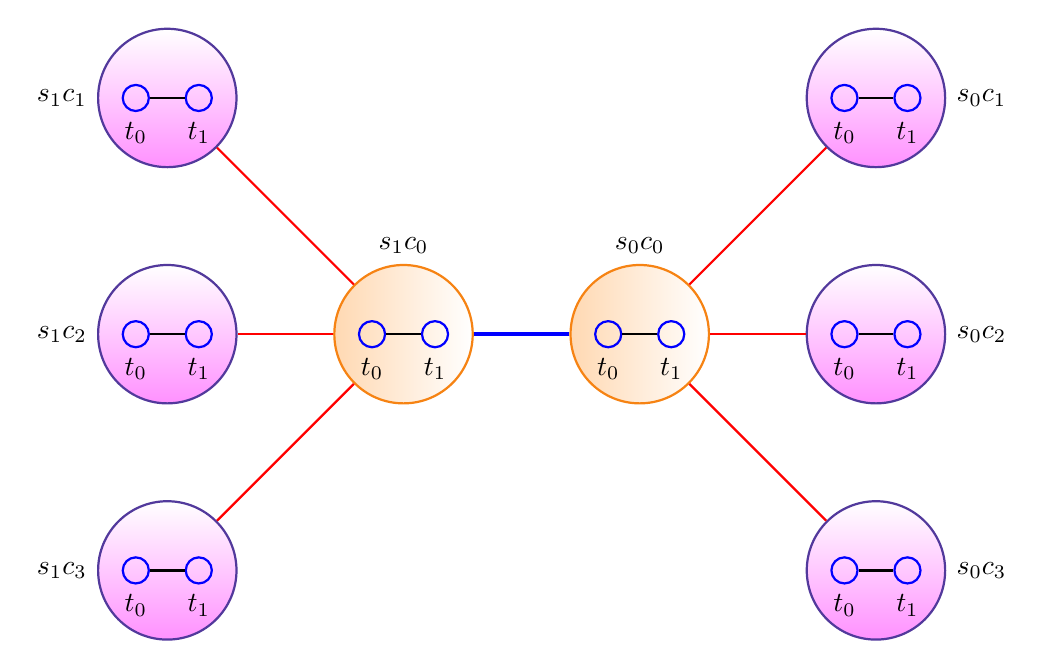
\begin{tikzpicture}[auto, thick]
  % Place base case
  \node[base,label=above:$s_0c_0$] (s0c0) at (1,0) {};
  \node[time,label=below:$t_0$] (s0c0t0) at (0.6,0) {};
  \node[time,label=below:$t_1$] (s0c0t1) at (1.4,0) {};
  
  \node[contingency,label=right:$s_0c_1$] (s0c1) at (4,3) {};
  \node[time,label=below:$t_0$] (s0c1t0) at (3.6,3) {};
  \node[time,label=below:$t_1$] (s0c1t1) at (4.4,3) {};

  \node[contingency,label=right:$s_0c_2$] (s0c2) at (4,0) {};
  \node[time,label=below:$t_0$] (s0c2t0) at (3.6,0) {};
  \node[time,label=below:$t_1$] (s0c2t1) at (4.4,0) {};

  
  \node[contingency,label=right:$s_0c_3$] (s0c3) at (4,-3) {};
  \node[time,label=below:$t_0$] (s0c3t0) at (3.6,-3) {};
  \node[time,label=below:$t_1$] (s0c3t1) at (4.4,-3) {};
  
  \path (s0c0t0) edge (s0c0t1);
  \path (s0c1t0) edge (s0c1t1);
  \path (s0c2t0) edge (s0c2t1);
  \path (s0c3t0) edge (s0c3t1);
  
  \path[cedge] (s0c0) edge (s0c1);
  \path[cedge] (s0c0) edge (s0c2);
  \path[cedge] (s0c0) edge (s0c3);

  % Second scenario
  \node[base,label=above:$s_1c_0$] (s1c0) at (-2,0) {};
  \node[time,label=below:$t_0$] (s1c0t0) at (-2.4,0) {};
  \node[time,label=below:$t_1$] (s1c0t1) at (-1.6,0) {};
  
  \node[contingency,label=left:$s_1c_1$] (s1c1) at (-5,3) {};
  \node[time,label=below:$t_0$] (s1c1t0) at (-5.4,3) {};
  \node[time,label=below:$t_1$] (s1c1t1) at (-4.6,3) {};

  \node[contingency,label=left:$s_1c_2$] (s1c2) at (-5,0) {};
  \node[time,label=below:$t_0$] (s1c2t0) at (-5.4,0) {};
  \node[time,label=below:$t_1$] (s1c2t1) at (-4.6,0) {};

  
  \node[contingency,label=left:$s_1c_3$] (s1c3) at (-5,-3) {};
  \node[time,label=below:$t_0$] (s1c3t0) at (-5.4,-3) {};
  \node[time,label=below:$t_1$] (s1c3t1) at (-4.6,-3) {};
  
  \path (s1c0t0) edge (s1c0t1);
  \path (s1c1t0) edge (s1c1t1);
  \path (s1c2t0) edge (s1c2t1);
  \path (s1c3t0) edge (s1c3t1);
  
  \path[cedge] (s1c0) edge (s1c1);
  \path[cedge] (s1c0) edge (s1c2);
  \path[cedge] (s1c0) edge (s1c3);

  \path (s0c0) edge [ultra thick,color=blue] (s1c0);

\end{tikzpicture}

\caption{Stochastic multi-period contingency constrained structure with two scenarios $s_0$ and $s_1$. Each scenario has three contingencies $c_1$,$c_2$,and $c_3$. $s_0c_0$ and $s_1c_0$ denote the base-cases for the two scenarios. Each scenario and contingency has two time-periods $t_0$, and $t_2$, $t_2$. The {\textcolor{red}{red}} line denotes the coupling between the contingencies and their respective base-case scenarios.The {\textcolor{blue}{blue}} line denotes the coupling between the scenarios}
\label{fig:sctopflow}
\end{figure}


The formulation for the stochastic security-constrained multi-period optimal power flow is given in (\ref{eq:sctopflow_start}) -- (\ref{eq:sctopflow_end}). In this formulation, the objective is to reduce the expected cost, where $f(x_{s,0,0})$ is the cost for scenario $s$ with no contingencies (hence 0 for the contingency index). $\rho_s$ is the probability of scenario $s$.

\begin{align}
\centering
\text{min}&~\sum_{s=1}^{N_s-1}\rho_s\sum_{c=0}^{N_c-1}\sum_{t=0}^{N_t-1}f(x_{s,c,t})&  \label{eq:sctopflow_start}\\
&\text{s.t.}& \nonumber \\
&~g(x_{s,c,t}) = 0,                                        &s \in \left[1,N_s-1\right],c \in \left[0,N_c-1\right], t \in \left[0,N_t-1\right]& \\
&~h(x_{s,c,t}) \le 0,                                      &s \in \left[1,N_s-1\right],c \in \left[0,N_c-1\right], t \in \left[0,N_t-1\right]& \\
x^- & \le x_{s,c,t} \le x^+,                               &s \in \left[1,N_s-1\right],c \in \left[0,N_c-1\right], t\in \left[0,N_t-1\right]& \\
-\delta_t{x} & \le x_{s,c,t} - x_{s,c,t-\Delta{t}} \le \delta_t{x},&s \in \left[1,N_s-1\right],c \in \left[0,N_c-1\right], t \in \left[1,N_t-1\right]& \label{eq:sctopflow_time_coupling}\\
-\delta_c{x} & \le x_{s,c,0} - x_{s,0,0} \le \delta_c{x},&s \in \left[1,N_s-1\right],c \in \left[1,N_c-1\right]&
\label{eq:sctopflow_contingency_coupling} \\
-\delta_s{x} & \le x_{s,0,0} - x_{0,0,0} \le \delta_s{x},&s \in \left[1,N_s-1\right]&
\label{eq:sctopflow_end}
\end{align}

{\sopflow} uses all the modeling details used for modeling an optimal power flow problem, i.e., each of the circles shown in Fig. \ref{fig:sctopflow} has the modeling details of an optimal power flow problem (\opflow). Incorporating the probabilities into the objective is one of the future action items. 

Currently, \sopflow uses wind power generation as the stochastic variables and each scenario is a realization of the power output from wind generators. A zero fuel cost is used for wind power generation to ensure wind generation would be the dispatched to the given target level (upper limit). 

For contingencies, \sopflow supports generation and/or transmission outages. A contingency can have multiple outages, but, it should not cause any islanding. The coupling between the no-contingency and the contingency case for each scenario is also the difference in real power output ($p_{jsct}^{\text{g}} - p_{js0t}^{\text{g}},~ \jinJgen$) that must be within the 30 minute generator ramp rate.

For multi time-period, we use ramping constraints on the generator real power output between successive time steps.

\sopflow can be run in two modes: preventive and corrective. In the preventive mode, generator real power output is fixed to the base-case values for generators at PV bus(es). In this mode, the generators at the reference bus provide/absorb any deficit/surplus power. The corrective mode allows deviation of the PV and PQ generator real power from the base-case dispatch constrained by its 30-min. ramp rate capability. Note that the preventive/corrective mode is only applied at the first step $t_0$. In the successive time-steps, the generator dispatch is dictated by the previous step dispatch and the ramp limits.

\section{Input and Output}
The following files are needed for executing a SOPFLOW.
\begin{itemize}
    \item \textbf{Network file:} The network file describing the network details. Only \matpower format files are currently supported.
    \item \textbf{Scenario file:} \sopflow only supports reading wind generation scenarios in a CSV format. An example of this format for the 9-bus case is \href{https://gitlab.pnnl.gov/exasgd/frameworks/exago/-/tree/master/datafiles/case9/scenarios.csv}{here}.
    \item \textbf{Contingency file:} Contingencies can be specified via PTI format file as described in chapter \ref{chap:scopflow}.The option \lstinline{-sopflow_enable_multicontingency} should be set for multi-contingency problems.
    \item \textbf{Load data:} One file for load real power and one fo reactive power. The files need to be in CSV format. An example of the format for the 9-bus case is \href{https://gitlab.pnnl.gov/exasgd/frameworks/exago/-/tree/master/datafiles/case9}{here}.
\end{itemize}

The \sopflow output is saved to a directory named \emph{sopflowout}. This directory contains $N_s$ subdirectories to save the solution for each scenario. Each of these subdirectories contain $N_c$ subdirectories, one for each contingency. Each contingency subdirectory has $N_t$ MATPOWER format files to store the output for each time-period for the given contingency and scenario. The subdirectories have the directory name format \emph{scen\_x} where x is the scenario number,  \emph{cont\_y} where y is the contingency number, and the output files have the file name format \emph{t\_z} where z is the time-step number.

\section{Solvers}
\sopflow can be solved with \ipopt. If one wants to solve each scenario independently, i.e., without any coupling constraints then use \emph{EMPAR} solver. \emph{EMPAR} distributes the contingencies to different processes when executed in parallel.
\section{Options}
See table \ref{tab:sopflow_options}

\begin{table}[h]
  \caption{SOPFLOW options}
  \small
  \begin{tabular}{|p{0.4\textwidth}|p{0.3\textwidth}|p{0.3\textwidth}|}
    \hline
    \textbf{Option} & \textbf{Meaning} & \textbf{Values (Default value)} \\ \hline
    -netfile & Network file name & string (\href{https://gitlab.pnnl.gov/exasgd/frameworks/exago/-/blob/master/datafiles/case9/case9mod_gen3_wind.m}{case9mod_gen3_wind.m}) \\ \hline
    -scenfile & Scenario file naame & string (\href{https://gitlab.pnnl.gov/exasgd/frameworks/exago/-/blob/master/datafiles/case9/scenarios.csv}{scenarios.csv}) \\ \hline
    -sopflow\_mode & Operation mode: Preventive or corrective & 0 or 1 (0) \\ \hline
    -sopflow\_enable\_multicontingency & Multi-contingency SOPFLOW & TRUE or FALSE (FALSE) \\ \hline 
  \end{tabular}
  \label{tab:sopflow_options}
\end{table}

With multi-contingency SOPFLOW, all \scopflow options given in Table \ref{tab:scopflow_options} can be used to tune the contingencies.

Depending on the \emph{mode}, SOPFLOW can either be \emph{preventive} (mode = 0) or \emph{corrective} (mode = 1). In the preventive mode, the PV and PQ generator real power is fixed to its corresponding base-case values. The generators at the reference bus pick up any make-up power required for the contingency. The corrective mode allows deviation of the PV and PQ generator real power from the base-case dispatch constrained by its 30-min. ramp rate capability.

\section{Usage}
\begin{lstlisting}
    ./sopflow -netfile <netfilename>  -scenfile <scenfilename> <sopflowoptions>
\end{lstlisting}
\section{Examples}
